\chapter{Existent infrastructure}

Before discussing solutions to these challenges, we must understand the current situation and constraints to which our
remote metering system must comply:

\begin{itemize}
    \item Absence of electricity at the site of deployment: we must produce the electricity required to run the system with some off-grid technology,
          for example solar panels. During certain weather conditions like snowfall, solar power might be unavailable for a longer period
          than battery power can last and the system
          must be able to hibernate and restart without manual intervention.
    \item Absence of reliable wireless infrastructure: The collected data must be transmitted to a location where
          it can be stored and analyzed. Network coverage at the site of deployment turns out to be week and
          unreliable.  The system must be able to cope with the inability to transfer measurements at a certain of point of  time
          and adopt some strategy of retrial without introducing measurement errors.
    \item how to interface with the current water meter ?
\end{itemize}

Let's start with the last point and have a closer look at what we have at the deployment site.

\section{Existent water meter}

The existent water meter installed upstream of the distribution network is shown in Fig \ref{fig:ewm}.
All drinking water headed towards the village passes through this meter, thus the totalizer on top of
the device shows to total consumption with a resolution of 1 l. The device is sealed and
the small reflective, revolving disc segment shown in Fig \ref{fig:totd} is made of non-magnetic material to avoid tampering,
emphasized within the red-bordered ellipse on the photo.

\begin{figure}[h]
    \centering
    \begin{subfigure}[b]{0.3\textwidth}
        \centering
        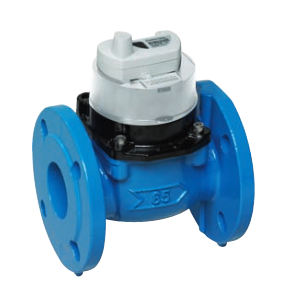
\includegraphics[width=\textwidth]{meter}
        \subcaption{WOLTEX M water meter}
        \label{fig:wwm}
    \end{subfigure}
    \hfill
    \begin{subfigure}[b]{0.3\textwidth}
        \centering
        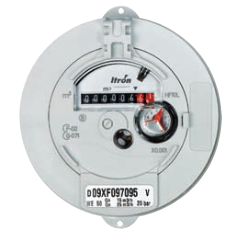
\includegraphics[width=\textwidth]{meter-detail}
        \subcaption{totalizer}
        \label{fig:tot}
    \end{subfigure}
    \hfill
    \begin{subfigure}[b]{0.3\textwidth}
        \centering
        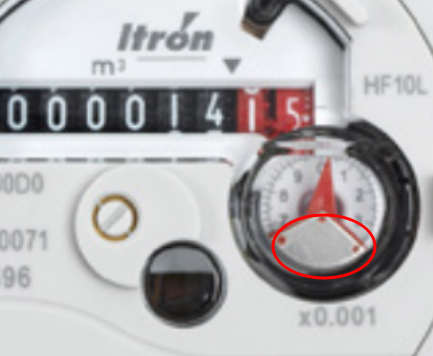
\includegraphics[width=\textwidth]{meter-detail-detail}
        \subcaption{totalizer detail}
        \label{fig:totd}
    \end{subfigure}
    \caption{The existent water meter}
    \label{fig:ewm}
\end{figure}

The manufacturer offers three different communication facilities:
\begin{enumerate}
    \item walk-by and drive by systems
    \item pulse output
    \item radio frequency LoRaWAN and Sigfox networks
\end{enumerate}


Option 1 is not practical because of the requirement to automatically detect possible leaks.
This must be done on a permanent basis without human intervention. The second option would require some investment to
change or unblock the current configuration. This is certainly possible, and it would have been the ideal option
for this use-case. However, there exist many older meters in the area without that feature and I believe that
it is interesting to develop techniques that can be used in conjunction with older analog devices.
Finally, the last options, LORaWAN and Sigfox both require additional network infrastructure (and electricity) to connect to
the Internet. When we started this project, LORaWAN was relatively new and the realistic range of radio coverage
in a mountainous and forested environment was unclear. Also, LoRaWAN - internet gateways were relatively expensive and
complicated to configure. Sigfox is a proprietary network owned by UnaBiz and for reasons already mentioned, we
strongly prefer open-source solutions.


We therefore choose to interface with the current meter via opto-coupling. In fact the totalizer shown in Fig \ref{fig:totd}
can be used to trigger an optical sensor, for example an optical switch.

We can now propose a system that fits into the current environment.

